\begin{figure}
\centering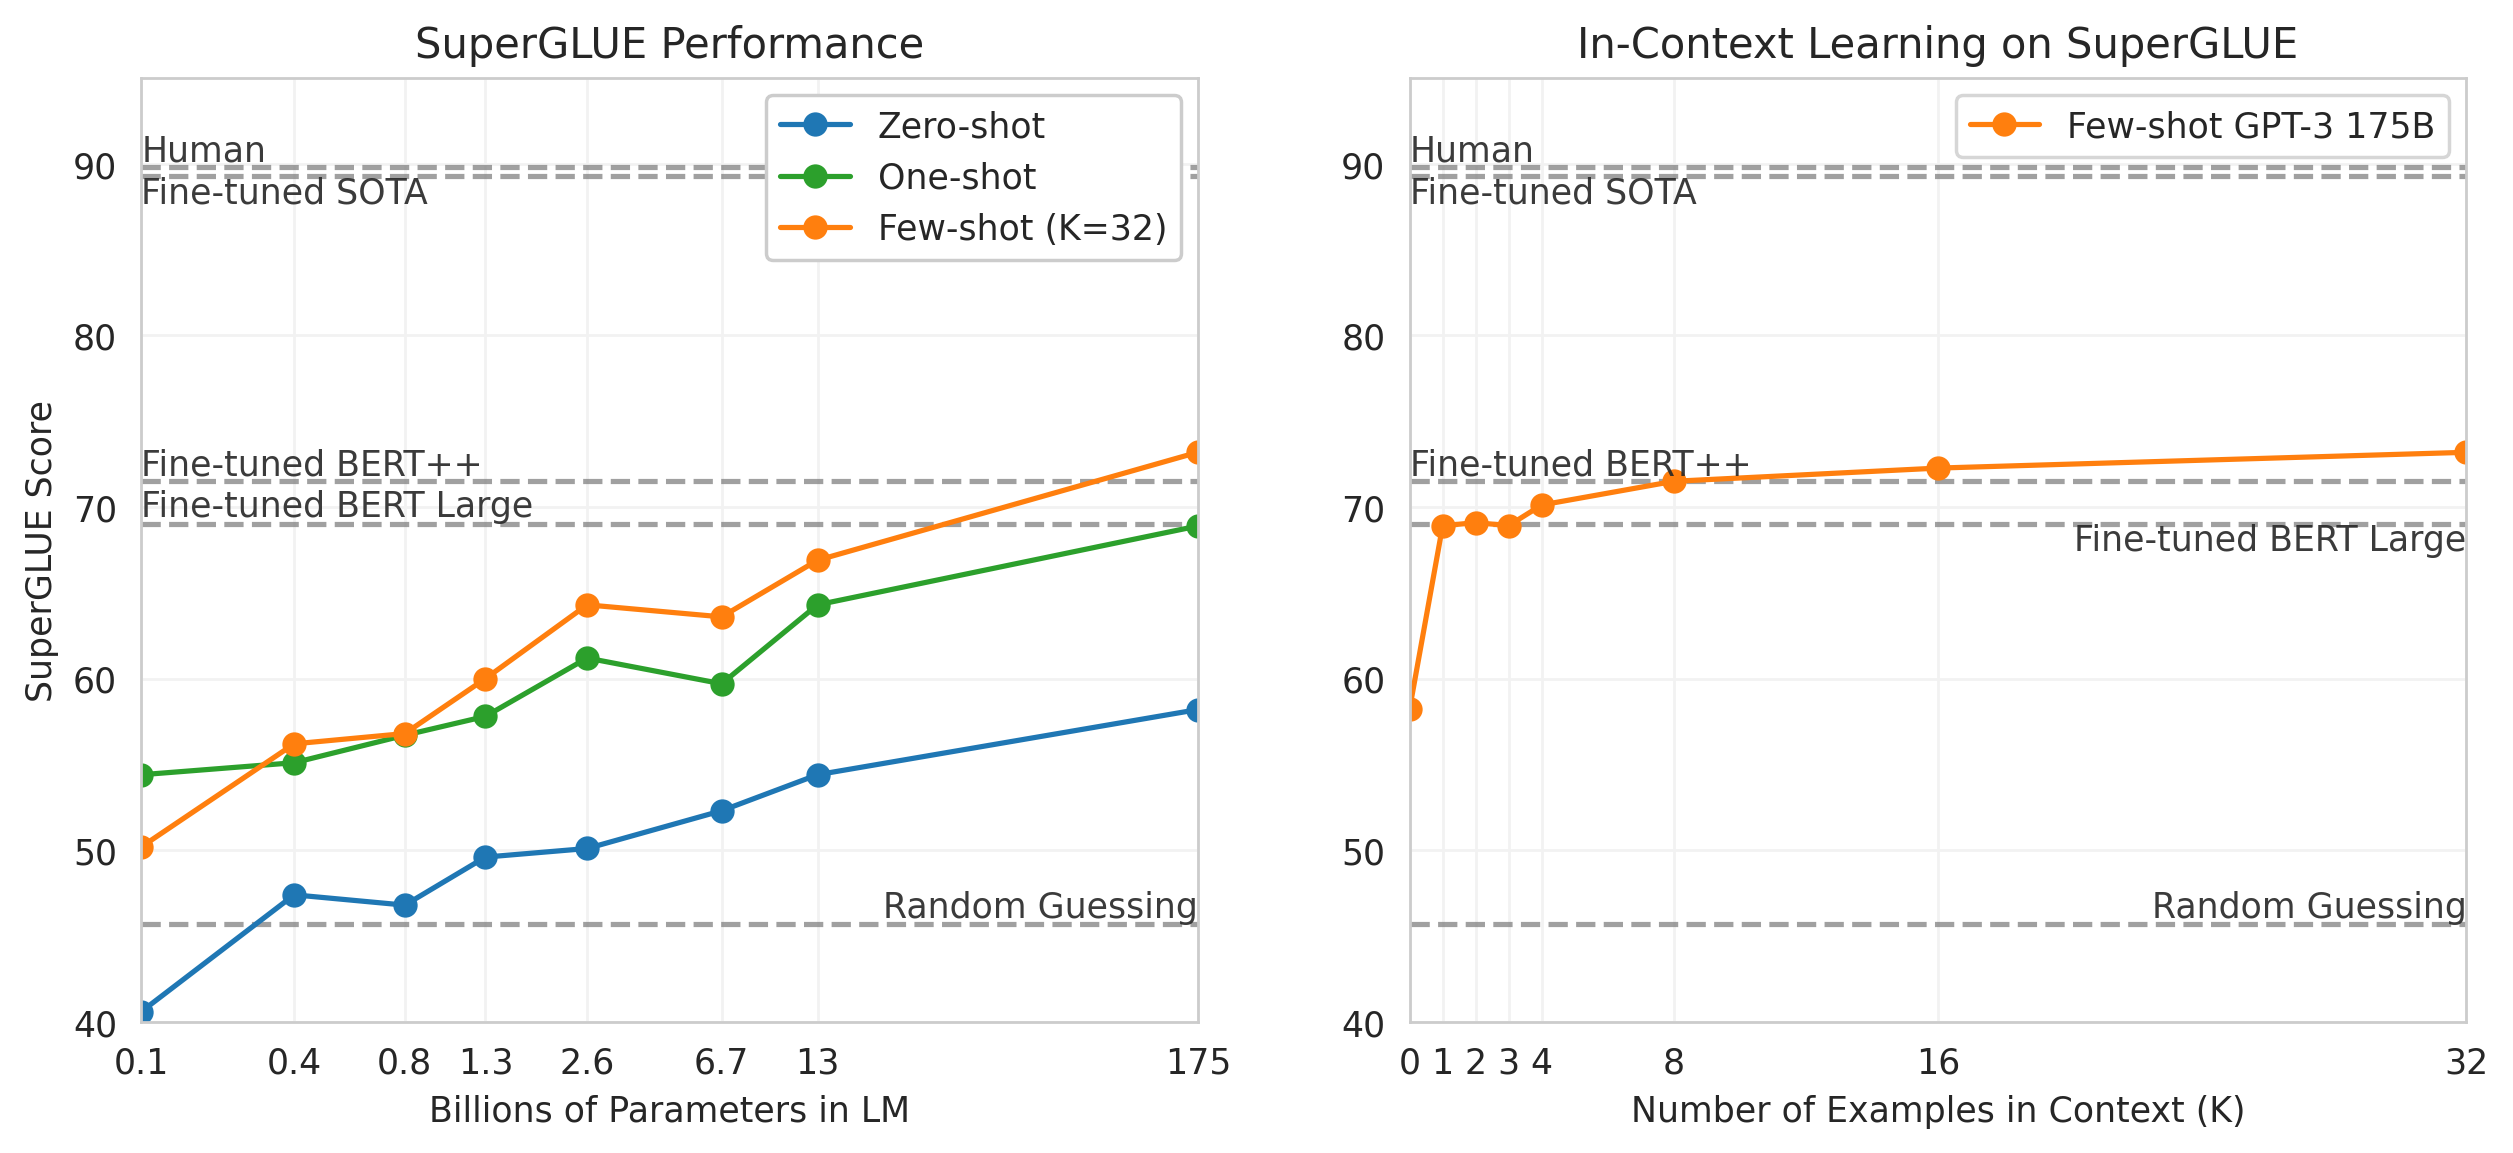
\includegraphics[width=1.0\linewidth]{figures/superglue_analysis.png}
\caption{
\textbf{
Performance on SuperGLUE increases with model size and number of examples in context.} A value of $K=32$ means that our model was shown 32 examples per task, for 256 examples total divided across the 8 tasks in SuperGLUE. We report GPT-3 values on the dev set, so our numbers are not directly comparable to the dotted reference lines (our test set results are in Table \ref{table:superglue}). The BERT-Large reference model was fine-tuned on the SuperGLUE training set (125K examples), whereas BERT++ was first fine-tuned on MultiNLI (392K examples) and SWAG (113K examples) before further fine-tuning on the SuperGLUE training set (for a total of 630K fine-tuning examples). We find the difference in performance between the BERT-Large and BERT++ to be roughly equivalent to the difference between GPT-3 with one example per context versus eight examples per context.
}
\label{graph:superglue_analysis}
\end{figure}
